\documentclass[../main.tex]{subfiles}

\begin{document}
    I hope the results more or less speak for themselves: I (or you) can write a document across multiple source files, avoiding the need to work in one huge file.

    Admittedly, this is just a game of mental organization.  But so is all of human thought beyond ``Grug hungry.  Grug eat food'', shortly after which Grug dies because he didn't have the mental organization to recognize a poisonous mushroom, like those shown in \autoref{fig:log}.

    To form only a slightly more articulate defense of mental organization: the efficient and correct consideration of ideas is probably the most important ability that seperates us from animals that have not achieved the same level of societal development as us.  You ought to think the organization of thoughts is important, and how you write things down is second only to how you organize your mind.

    \subsection{A Picture of a Log}
    \begin{figure}[h!]
        \centering
        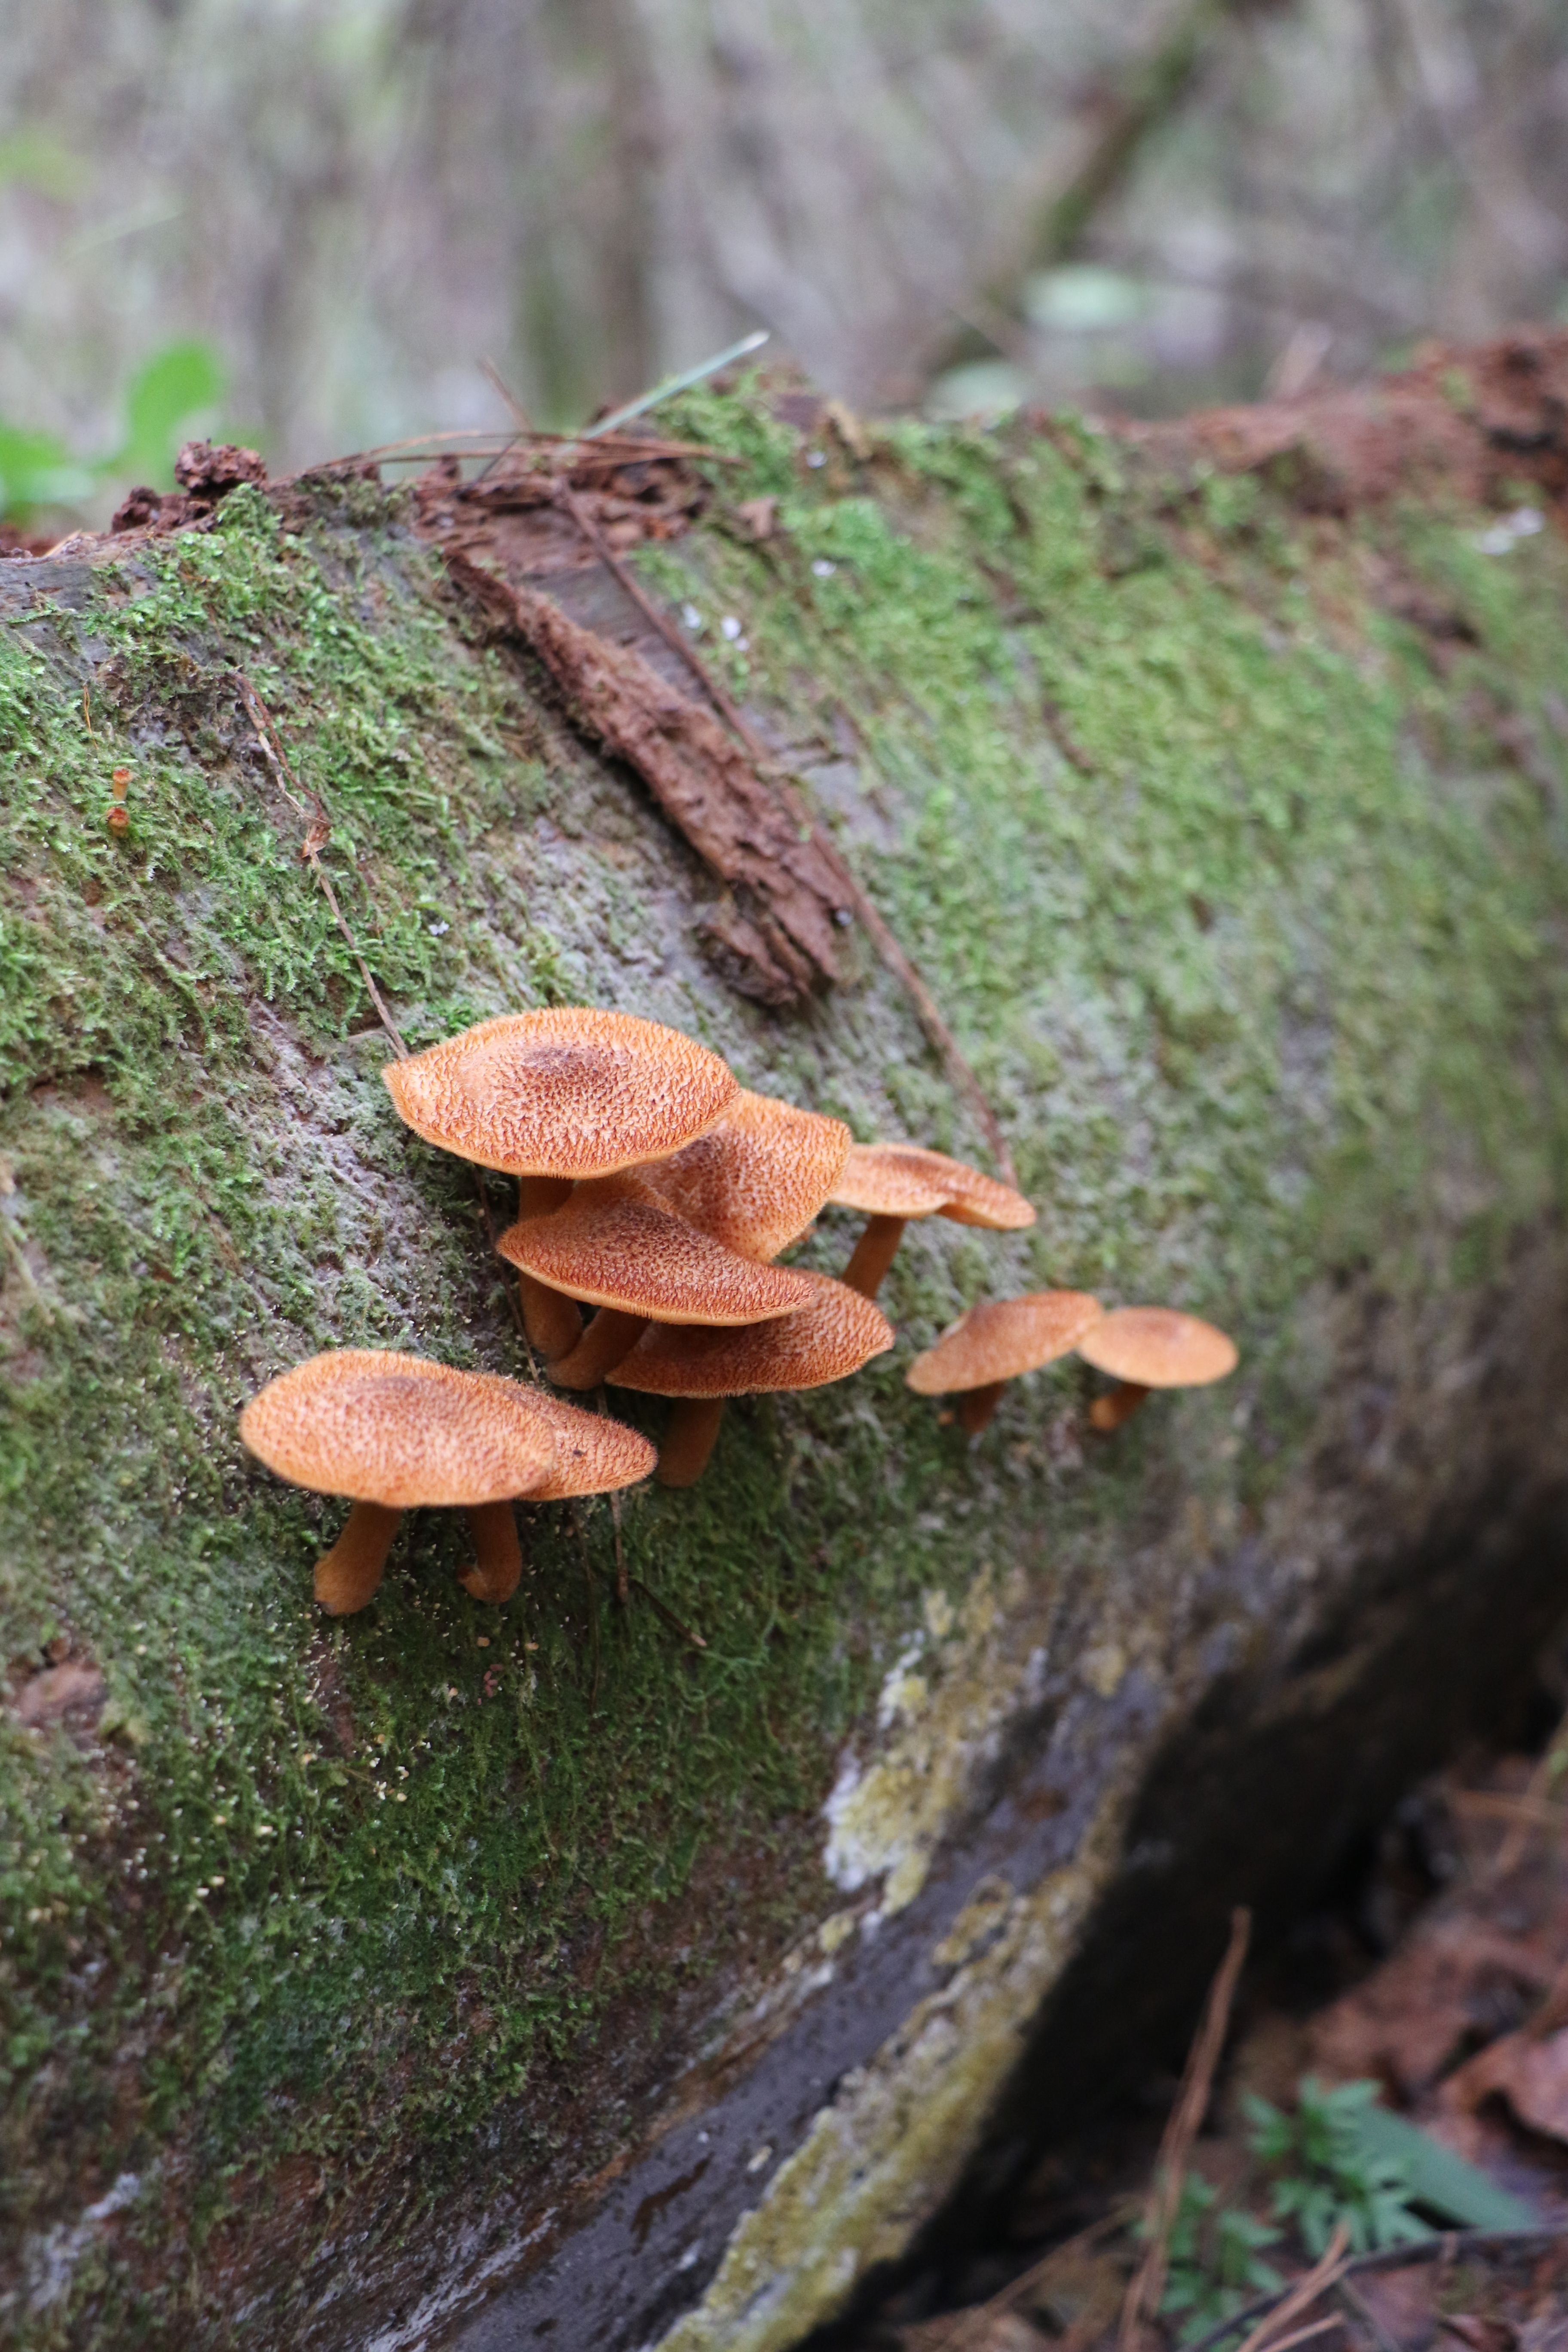
\includegraphics[width=0.6\textwidth]{../figures/results/log.jpg}
        \caption{An image of a log.}
        \label{fig:log}
    \end{figure}

    \subsection{Lipsum Text, Section III}
    \lipsum[3]
\end{document}
